\lstinputlisting[language=bash,basicstyle=\small]{python_codes/fieldstone_68/keywords}

\begin{center}
Code at \url{https://github.com/cedrict/fieldstone/tree/master/python_codes/fieldstone_68}
\end{center}

\par\noindent\rule{\textwidth}{0.4pt}

%%%%%%%%%%%%%%%%%%%%%%%%%%%%%%%%%%%%%%%%%%%%%%%%%%%%%%%%%%%%%%%%%%%%%%%%%%%%%%%%%%%%%%%%%%%%%%%%%%%%


\Literature: \cite{vack08}\cite{syva10}\cite{vakn12}


%------------------------------------------------------------
\subsubsection*{Description of the setup and benchmark cases}


The domain is $660\text{km}\times 600\text{km}$. 

\begin{center}
\includegraphics[width=14cm]{python_codes/fieldstone_68/images/fig1}\\
{\captionfont Taken from van Keken et al (2008) \cite{vack08}.
(a) Cartoon of the cornerflow model for subduction zone dynamics. 
(b) Benchmark geometry of a kinematic slab driving flow in the viscous
mantle wedge below a rigid overriding plate. 
(c) Boundary conditions for Stokes and temperature equations.}
\end{center}

As shown in the figure above, 
the inflow boundaries (at both wedge and trench sides) and top of the model 
have prescribed temperature. The wedge is assumed to be an incompressible fluid that
is driven only by the kinematic forcing of the slab. The wedge is
confined by the top of the slab and the base of the rigid overriding
plate (located at a depth of $50\text{km}$). 
The boundary conditions for the wedge are no-slip below the overriding plate and constant velocity
along the top of the slab. The velocity boundary conditions for the
boundaries of the wedge are either provided by the Batchelor cornerflow 
solution (cases 1a and 1b) or based on free inflow/outflow
boundaries (cases 1c, 2a, 2b). The velocity field is discontinuous between the slab
and the overriding plate.
The velocity in the slab is constant (5cm/yr) and it dips at a $45\degree$ angle
There is no radiogenic of shear heating.
The mantle wedge rheology is either linear viscous (cases 1a,b,c),
diffusion creep (case 2a) or dislocation creep (case 2b).





%___________________
\paragraph{Case 1a} The Stokes equations are not solved. Instead the velocity field
is prescribed analytically everywhere in the domain, using the corner flow solution 
in the mantle wedge. 

%___________________
\paragraph{Case 1b - dynamical flow in isoviscous wedge I}
This case is the same as 1a, except that the solution
for the wedge flow is determined by solving the Stokes equations while the Batchelor solution is
imposed on the inflow and outflow boundaries. This case tests the ability of the numerical method
to accurately reproduce the corner flow solution.



%___________________
\paragraph{Case 1c - dynamical flow in isoviscous wedge II} 
Same as case 1b, but with stress-free boundary conditions on the mantle wedge.



%___________________
\paragraph{Case 2a}

This case is the same as 1c, except that the viscosity of the wedge
is given by 
\[
\eta_{\text{diff,eff}} = \left( \frac{1}{\eta_{\text{diff}}} + \frac{1}{\eta_{\text{max}}} \right)^{-1}
\]
and
\[
\eta_{\text{diff}}=A_{\text{diff}} \exp\left( \frac{Q_{\text{diff}}}{RT} \right)
\]
with
$Q_{diff}=335kJ/mol$ and $A_{diff}=1.32043 \cdot 10^9Pa\cdot s$. $\eta_{max}=10^{26}$Pa.s

%___________________
\paragraph{Case 2b}

This case is the same as 1c, except that the viscosity of the wedge
is given by 
\[
\eta_{\text{disl,eff}} = \left( \frac{1}{\eta_{\text{disl}}} + \frac{1}{\eta_{\text{max}}} \right)^{-1}
\]
and
\[
\eta_{\text{disl}}=
A_{\text{disl}} \dot\varepsilon^{(1-n)/n} \exp \left( \frac{Q_{\text{disl}}}{nRT} \right)
\]
with $Q_{\text{disl}}=540kJ/mol$, $n=3.5$ and $A_{\text{disl}}=28968.6Pa\cdot s^{1/n}$. 
$\eta_{\text{max}}=10^{26}$Pa.s





%------------------------------------------------------------
\subsubsection*{Building a mesh}

The mesh is built using Gmsh \cite{gere09}. Here, we briefly describe the steps required 
to make a generic subduction geometry mesh. This workflow can be easily adapted to any 
complex subduction geometry desired. 

The first step towards building a mesh with Gmsh is to make a .geo file, which sets up the 
entire mesh. Here, we provide a meshing script {\sl make\_mesh.py} that makes a .geo file for you. 
To get the {\sl make\_mesh.py} script to work, all you need is a file with a predefined 
subduction geometry with the first column indicating all the $x$-coordinates in km 
with the convention that the positive $x$-axis is towards the right and the 
second column indicating the $y$-coordinates in km with the convention that the $y$-axis 
is positive downwards. In the file {\sl geometry\_van\_keken.txt}, 
the simple geometry required for the \cite{vack08} benchmark is provided, but any subduction geometry will do.


In the input section of {\sl make\_mesh.py}, the model dimensions and resolution of different 
sections of the mesh can be changed. After that, the script dives into writing the .geo 
file. The .geo file starts by defining the different resolutions that will be used throughout the mesh. 
Then, all the points in the mesh (i.e., those setting up the model domain and the subduction geometry) 
are written including the desired resolution at each point. This way, we can easily define a high 
resolution at the subduction interface and a lower resolution in parts of the mantle (i.e., lower left corner). 

We add additional points in the mesh to form a subduction channel (its width can be specified 
in the input parameters) to deal with the discontinuity in kinematically described velocities 
on the downgoing plate interface and the overriding plate at the interface between the two. 

After describing all the points in the mesh, we define the relevant lines in the mesh by connecting 
two points. We add flags (i.e., specific numbers) to certain lines to simplify setting the boundary 
conditions in fieldstone. For example, we give the 101 flag to all lines that together create the 
top of the subducting plate, so that we know that we have to impose a velocity to all element edges 
with a 101 flag.

We then create a closed loop of the lines (a line loop) for each area in the mesh. Note that all the line loops are created counterclockwise. Consistency in the direction of the lines loops is important to preserve sign consistency of all areas across the mesh. This is handy when setting up the surfaces later. Correct signs of line loops become increasingly important when going towards three-dimensional meshes. Also note that to set up line loops correctly, the individual lines need to have the correct direction as well. For example, line number 1 which might be defined as the line from point 1 to point 2, should be called line number -1 when the line from point 2 to point 1 is required in the line loop. 

After making the line loops, each line loop is made into a plane surface. Combining these separate plane surfaces into a physical surface completes the mesh setup. 

We add one additional line to the mesh for the plane surface of the subduction channel:

MeshAlgorithm Surface\{2000000\} = 3;

This ensures that the width of the channel is always one element, which reduces the amount of miniconvection cells in the channel in the vicinity of contrasting kinematic boundary conditions at the interface between the subducting slab and the overriding plate. 

So, now you can run
(make sure that {\sl geometry\_van\_keken.txt} is in the same folder as {\sl make\_mesh.py})
\begin{verbatim}
> python3 make_mesh.py
\end{verbatim}
and the script produces the {\sl vankeken.geo} file. 

You can open this .geo file in Gmsh version 4.5.6 or later (earlier versions will not support the 
last line in the .geo script describing the one-element wide area). To produce the mesh in 
the Gmsh GUI, click on `mesh', and then `2D'. To increase the order of the 
elements (as needed by fieldstone), click `Set order 2'. To save the mesh in the 
format that fieldstone can handle, click on `File $>$ Export' and choose extension `Mesh - Gmsh MSH (*.msh)'. 
In the little pop-up box with options, choose `Version 2 ASCII' and click `OK'. This will then 
produce a .msh file that can be read in and used by fieldstone. 

\begin{center}
\includegraphics[width=13cm]{python_codes/fieldstone_68/images/gmsh}\\
{\captionfont Screen capture of the Gmesh interface}
\end{center}


\begin{center}
\includegraphics[width=7cm]{python_codes/fieldstone_68/images/mesh1}
\includegraphics[width=7cm]{python_codes/fieldstone_68/images/mesh2}\\
{\captionfont Details of the mesh as seen in Paraview.}
\end{center}

\begin{center}
\includegraphics[width=7cm]{python_codes/fieldstone_68/images/interfaces}
\end{center}

%..........................................
\subsubsection*{Description of the code}


Crouzeix-Raviart elements are used for the Stokes equations (see Section~\ref{sec:crouzeix-raviart}) 
and $P_2$ elements are used for the temperature. 

The origin of the coordinate system $(x,y)$ is at the top left, i.e. $y$ is negative. The boundary conditions for the
wedge are no-slip below the overriding plate and constant velocity along the top of the slab. 
The velocity boundary conditions for the boundaries of the wedge are either provided by the Batchelor 
cornerflow solution (cases 1a and 1b) or based on free inflow/outflow boundaries. 
The velocity field is discontinuous between the slab and the overriding plate which effectively mimics the fault 
representative of the seismogenic zone in subduction zones.

For cases 1a,b,c the Stokes equations and the energy equation are not really coupled: the gravity is set to zero, the 
model is driven by the kinematical boundary conditions and the viscosity is constant, so that temperature does not 
influence the Stokes solve. Once the velocity field is obtained it is used in the energy equation to compute the 
steady state temperature field. 

For cases 2a,b the viscosity of the mantle 
wedge is temperature (and strain rate) dependent so that the coupling of the PDEs 
requires nonlinear iterations. These are as follows:
\begin{enumerate}
\item set $\vec{\upnu}_{old}$=0, $T_{old}=0$ at all mesh nodes.
\item Solve Stokes equation with $\eta(T_{old},\dot{\varepsilon}_{old})$ (if iter=0, use $\eta=10^{21}$ for the whole domain).
\item Relax the velocity solution: $\vec\upnu = relax \cdot \vec{\upnu} + (1-relax)\cdot \vec{\upnu}_{old}$
\item Solve for temperature 
\item Relax the temperature solution: $T=relax \cdot T + (1-relax) \cdot T_{old}$
\item Check for convergence. If $\|\vec\upnu-\vec\upnu_{old}\|_2 < tol \| \vec\upnu + \vec\upnu_{old}  \|_2$ and 
$\|T-T_{old}\|_2 < tol \| T + T_{old}  \|_2$ then exit, otherwise: $T_{old} \leftarrow T$, $ \vec\upnu \leftarrow \vec\upnu_{old} $. iter+=1. Go back to 2. 
\end{enumerate}

The $relax$ parameter should obviously be between 0 and 1. 

To compare model results each
group contributed the temperature field as discreted values $T_{ij}$ on
an equidistant grid with 6 km spacing, which is a 111x101 matrix
stored row-wise starting in the top left corner. 

\begin{center}
\includegraphics[width=5cm]{python_codes/fieldstone_68/images/grid1}
\includegraphics[width=5cm]{python_codes/fieldstone_68/images/grid2}\\
{\captionfont Measuring grid made of 110x100 points.}
\end{center}

From this grid we have extracted the following measurements for direct comparison:
\begin{itemize}
\item the temperature $T_{11,11}$ which is at coordinates (60, 60 km) and
just down-stream from the corner point.
\item the L2 norm of the slab–wedge interface temperature between
0 and 210 km depth defined by
\[
T_{slab} = \sqrt{\frac{1}{36} \sum_{i=1}^{36} T_{ii}^2  }
\]
\item 
the L2 norm of the temperature in the triangular part of the
tip of the wedge, between 54 and 120 km depth:
\[
T_{wedge} = \sqrt{ \frac{1}{78} \sum_{i=10}^{21} \sum_{j=10}^i T_{ij}^2   }
\]
\end{itemize}

\begin{center}
\includegraphics[width=5cm]{python_codes/fieldstone_68/images/grid3}
\includegraphics[width=5cm]{python_codes/fieldstone_68/images/grid4}
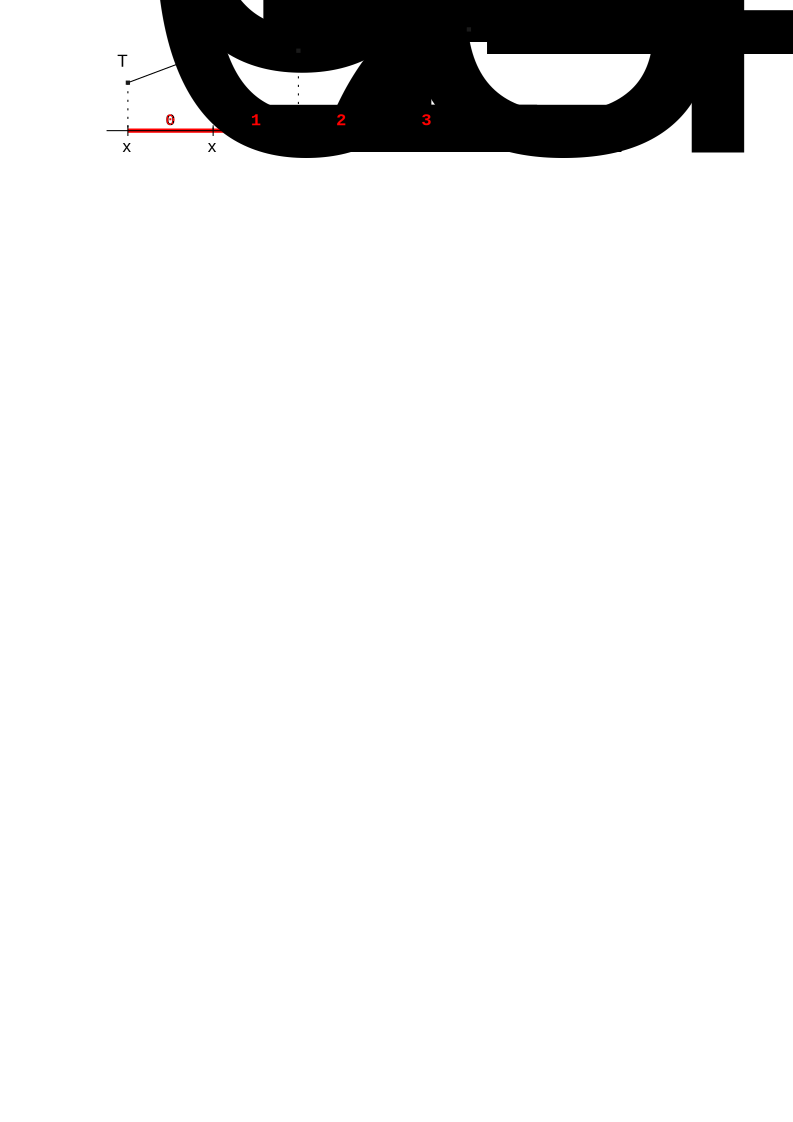
\includegraphics[width=5cm]{python_codes/fieldstone_68/images/grid5}\\
{\captionfont The black dots indicate the different types of reported quantities in the paper.}
\end{center}

In order to interpolate temperature on this grid, we need to find out in which 
triangle each point of the grid lies. This is a rather costly algorithm for now. 
In order to determine whether a point is inside a triangle, we assume that 
the reduced coordinates $r,s$ exist and satisfy the following 
relationships:
\begin{eqnarray}
x &=& N_1(r,s) x_1 + N_2(r,s) x_2 + N_3(r,s) x_3 \nn\\  
y &=& N_1(r,s) y_1 + N_2(r,s) y_2 + N_3(r,s) y_3 \nn
\end{eqnarray}
where $N_i$ are the linear basis functions inside a triangle, see Section~\ref{ss:p1}.

We also have the property that $N_1+N_2+N_3=1$ everywhere inside the element, so that 
we now have a system of 3 equations for our three unknowns $N_1$, $N_2$ and $N_3$ (having
obtained these, we can later easily find $r$ and $s$).
We must then solve:
\begin{eqnarray}
x &=& N_1 x_1 + N_2 x_2 + N_3 x_3 \nn\\  
y &=& N_1 y_1 + N_2 y_2 + N_3 y_3 \nn\\
0 &=& N_1+N_2+N_3 \nn
\end{eqnarray}
which yields
\[
N_1=\frac{(y_2 - y_3)(x - x_3) + (x_3 - x_2)(y - y_3)}{(y_2 - y_3)(x_1 - x_3) + (x_3 - x_2)(y_1 - y_3)}
\qquad
N_2=\frac{(y_3 - y_1)(x - x_3) + (x_1 - x_3)(y - y_3)}{(y_2 - y_3)(x_1 - x_3) + (x_3 - x_2)(y_1 - y_3)}
\qquad
N_3=1-a-b
\]
and then $r=N_2$ and $s=N_3$

%------------------------------------------------------------
\subsubsection*{Results}


%_______________________
\paragraph{Cases 1a,b,c}. 

\begin{center}
\includegraphics[width=14cm]{python_codes/fieldstone_68/images/fig2}\\
{\captionfont Taken from \cite{vack08}. Temperature prediction for case 1a. 
The bold lines indicate the top of the slab and base of the overriding plate. 
(b) Close up of the top left part of the model.}
\end{center}


\begin{landscape}
\begin{center}
1a:\includegraphics[width=5.3cm]{python_codes/fieldstone_68/results/case1a/T_1a}
\includegraphics[width=5.3cm]{python_codes/fieldstone_68/results/case1a/u_1a}
\includegraphics[width=5.3cm]{python_codes/fieldstone_68/results/case1a/v_1a}
\includegraphics[width=5.3cm]{python_codes/fieldstone_68/results/case1a/vel_1a}\\
1b:\includegraphics[width=5.3cm]{python_codes/fieldstone_68/results/case1b/T_1b}
\includegraphics[width=5.3cm]{python_codes/fieldstone_68/results/case1b/u_1b}
\includegraphics[width=5.3cm]{python_codes/fieldstone_68/results/case1b/v_1b}
\includegraphics[width=5.3cm]{python_codes/fieldstone_68/results/case1b/vel_1b}\\
1c:\includegraphics[width=5.3cm]{python_codes/fieldstone_68/results/case1c/T_1c}
\includegraphics[width=5.3cm]{python_codes/fieldstone_68/results/case1c/u_1c}
\includegraphics[width=5.3cm]{python_codes/fieldstone_68/results/case1c/v_1c}
\includegraphics[width=5.3cm]{python_codes/fieldstone_68/results/case1c/vel_1c}\\
{\captionfont From left to right: Temperature, $x-$ and $y-$component of the 
velocity and velocity field. Temperature isocontours are every 100$\degree$.}
\end{center}
\end{landscape}


\begin{landscape}
\includegraphics[width=11.5cm]{python_codes/fieldstone_68/images/fig3}
\includegraphics[width=11.5cm]{python_codes/fieldstone_68/results/van_keken_2008_fig3.jpg}\\
{\captionfont Left: Taken from \cite{vack08}. 
Predictions for selected thermal properties for the isoviscous benchmark cases 1a 
(frames a-c), 1b (d-f) and 1c (g-i). The quantities represent a spot measurement at
the slab–wedge interface at 60 km depth (frames a, d, g), the average temperature 
along the slab–wedge interface from 0 to 210 km depth (frames b, e, h), and the
average temperature in a triangular portion of the wedge (frames c, f, i). 
The averages are computed with an L2 norm from an equidistant grid with 6 km spacing.
Right: recreated figure with additional fieldstone results in yellow.
}
\end{landscape}

 
%_______________________
\paragraph{Cases 2a}.

\begin{center}
\includegraphics[width=14cm]{python_codes/fieldstone_68/images/fig4}\\
{\captionfont Taken from \cite{vack08}. 
(a) Temperature prediction for case 2a with olivine diffusion creep in 
the mantle wedge. (b) Close up of the top left part of the model, as in Fig. 2b.
}
\end{center}

\begin{center}
\includegraphics[width=5.cm]{python_codes/fieldstone_68/results/case2a/T}
\includegraphics[width=5.cm]{python_codes/fieldstone_68/results/case2a/u}
\includegraphics[width=5.cm]{python_codes/fieldstone_68/results/case2a/v}\\
\includegraphics[width=5.cm]{python_codes/fieldstone_68/results/case2a/vel}
\includegraphics[width=5.cm]{python_codes/fieldstone_68/results/case2a/e}
\includegraphics[width=5.cm]{python_codes/fieldstone_68/results/case2a/eta}\\
{\captionfont Case 2a. 4km resolution}
\end{center}

\begin{center}
\includegraphics[width=10cm]{python_codes/fieldstone_68/results/case2a/conv.pdf}\\
{\captionfont obtained with $tol=10^{-4}$}
\end{center}

\begin{center}
\includegraphics[width=3.74cm]{python_codes/fieldstone_68/results/case2a/eta0000}
\includegraphics[width=3.74cm]{python_codes/fieldstone_68/results/case2a/eta0009}
\includegraphics[width=3.74cm]{python_codes/fieldstone_68/results/case2a/eta0019}
\includegraphics[width=3.74cm]{python_codes/fieldstone_68/results/case2a/eta0028}\\
\includegraphics[width=3.74cm]{python_codes/fieldstone_68/results/case2a/T0000}
\includegraphics[width=3.74cm]{python_codes/fieldstone_68/results/case2a/T0009}
\includegraphics[width=3.74cm]{python_codes/fieldstone_68/results/case2a/T0019}
\includegraphics[width=3.74cm]{python_codes/fieldstone_68/results/case2a/T0028}\\
{\captionfont Quadrature points. Top row: viscosity; Bottom row: temperature.
from left to right: iteration 0,9,19,28.}
\end{center}


%_______________________
\paragraph{Cases 2b}.

The only visual we have from the paper itself for this case is the following picture:

\begin{center}
\includegraphics[width=5cm]{python_codes/fieldstone_68/images/fig4c}\\
{\captionfont Taken from \cite{vack08}. Close up of the model with olivine dislocation creep in the mantle wedge.}
\end{center}

\begin{center}
\includegraphics[width=10cm]{python_codes/fieldstone_68/results/case2b/conv.pdf}\\
{\captionfont obtained with $tol=10^{-4}$}
\end{center}

\begin{center}
\includegraphics[width=5.cm]{python_codes/fieldstone_68/results/case2b/T}
\includegraphics[width=5.cm]{python_codes/fieldstone_68/results/case2b/u}
\includegraphics[width=5.cm]{python_codes/fieldstone_68/results/case2b/v}\\
\includegraphics[width=5.cm]{python_codes/fieldstone_68/results/case2b/vel}
\includegraphics[width=5.cm]{python_codes/fieldstone_68/results/case2b/e}
\includegraphics[width=5.cm]{python_codes/fieldstone_68/results/case2b/eta}\\
{\captionfont Case 2a. 4km resolution}
\end{center}

\begin{landscape}
\includegraphics[width=8cm]{python_codes/fieldstone_68/images/fig5}
 + Iris figure soon
\end{landscape}




